\section{Preliminaries}
\label{sect:dssat-preliminaries}

\subsection{Dependency quantified Boolean formula}
\label{sect:dssat-dqbf}
DQBF is formulated as \textit{multiple-person alternation} by Peterson and Reif~\cite{Peterson1979}.
In contrast to the \textit{linearly ordered} quantification used in QBF,
i.e., an existentially quantified variable depends on all of its preceding universally quantified variables,
the quantification structure in DQBF is extended with \textit{Henkin quantifiers},
where the dependency of an existentially quantified variable is explicitly specified.

A DQBF $\Qf$ over a set $V=\{x_1,\ldots,x_n,y_1,\ldots,y_m\}$ of variables is of the form:
\begin{align*}
    \Qf=\forall x_1,\ldots,\forall x_n,\exists y_1(\dep{y_1}),\ldots,\exists y_m(\dep{y_m}).\pf(x_1,\ldots,x_n,y_1,\ldots,y_m),
\end{align*}
where each $\dep{y_j}\subseteq\{x_1,\ldots,x_n\}$ denotes the set of universally quantified variables that $y_j$ depends on,
and Boolean formula $\pf$ over $V$ is quantifier-free.
We denote the set $\{x_1,\ldots,x_n\}$ (resp. $\{y_1,\ldots,y_m\}$) of universally (resp. existentially) quantified variables of $\Qf$ by $\uvs$ (resp. $\evs$).

A DQBF $\Qf$ is satisfiable if for each variable $y_j$,
there exists a Boolean function $f_j:\av{\dep{y_j}}\mapsto\booldom$,
such that matrix $\pf$ becomes a tautology over $\uvs$
after substituting variables in $\evs$ with their respective Boolean functions.
The set $\skf=\{f_1,\ldots,f_m\}$ of Boolean functions is called a set of \textit{Skolem} functions for $\Qf$.
In other words, $\Qf$ is satisfied by $\skf$ if the following QBF valuates to $\top$:
\begin{align}
    \label{eq:dssat-dqbf-satisfiable}
    \forall x_1,\ldots,\forall x_n.\pf(x_1,\ldots,x_n,f_1,\ldots,f_m),
\end{align}
where $\pf(x_1,\ldots,x_n,f_1,\ldots,f_m)$ represents the formula obtained by substituting existentially quantified variables in $\pf$ with their respective Skolem functions.
We extend the notation for cofactors and denote $\pf(x_1,\ldots,x_n,f_1,\ldots,f_m)$ by $\pcf{\pf}{\skf}$.
The satisfiability problem of DQBF is NEXPTIME-complete \cite{Peterson2001}.

\subsection{Decentralized POMDP}
\label{sect:dssat-dec-pomdp}
Dec-POMDP is a formalism for multi-agent systems under uncertainty and with partial information.
Its computational complexity is NEXPTIME-complete~\cite{Bernstein2002}.
In the following, we briefly review the definition, optimality criteria,
and value function of Dec-POMDP from the literature~\cite{Oliehoek2016}.

A Dec-POMDP is specified by a tuple $\mathcal{M}=(I,S,\{A_i\},T,\rho,\{O_i\},\Omega,\Delta_0,h)$, where
$I=\{1,\ldots,n\}$ is a finite set of $n$ agents,
$S$ is a finite set of states,
$A_i$ is a finite set of actions of Agent $i$,
$T:S\times(A_1\times\cdots\times A_n)\times S\mapsto [0,1]$ is a transition distribution function with
$T(s,\Vec{a},s')=\Pr[s'|s,\vec{a}]$,
the probability to transit to state $s'$ from state $s$ after taking actions $\vec{a}$,
$\rho:S\times(A_1\times\cdots\times A_n)\mapsto\mathbb{R}$ is a reward function with
$\rho(s,\vec{a})$ giving the reward for being in state $s$ and taking actions $\vec{a}$,
$O_i$ is a finite set of observations for Agent $i$,
$\Omega:S\times(A_1\times\cdots\times A_n)\times(O_1\times\cdots\times O_n)\mapsto[0,1]$ is an observation distribution function with
$\Omega(s',\Vec{a},\vec{o})=\Pr[\vec{o}|s',\vec{a}]$,
the probability to receive observation $\vec{o}$ after taking actions $\vec{a}$ and transiting to state $s'$, $\Delta_0:S\mapsto [0,1]$ is an initial state distribution function with $\Delta_0(s)=\Pr[s^0 \equiv s]$,
the probability for the initial state $s^0$ being state $s$,
and $h$ is a planning horizon, which we assume finite in this work.

\begin{figure}[t]
    \centering
    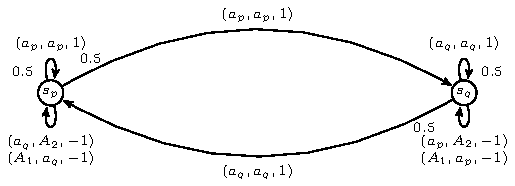
\includegraphics[scale=1.5]{fig/build/dec-pomdp-example.pdf}
    \caption{A two-agent Dec-POMDP example}
    \label{fig:dssat-dec-pomdp-state-graph}
\end{figure}

\begin{example}
    An example Dec-POMDP $\mathcal{M}$ with two agents and two states $s_p,s_q$
    is shown in~\cref{fig:dssat-dec-pomdp-state-graph}.
    The goal of the agents is to make a correct agreement on the current state.
    They have an action set $A_1=A_2=\{a_p,a_q\}$,
    where $a_p$ (resp. $a_q$) is used to guess that the current state is $s_p$ (resp. $s_q$).

    Under the assumption of partial observation, the agents cannot access the current state of $\mathcal{M}$.
    Instead, they have two different observations $o_p$ and $o_q$.
    We assume that an agent will receive $o_p$ (resp. $o_q$) after the current state transits to $s_p$ (resp. $s_q$) with probability $\Omega(s_p,o_p)$ (resp. $\Omega(s_q,o_q)$).

    If both agents guess correctly, they will receive a reward of $1$,
    and $\mathcal{M}$ will transit to a next state with equal probability.
    In the state-transition graph, observe that in state $s_p$ (resp. $s_q$),
    there are two outgoing edges labeled with a tuple $(a_p,a_p,1)$ (resp. $(a_q,a_q,1)$),
    which describes the agents' actions and the reward.
    These two edges will be taken with probability $0.5$ if the preconditions are met.

    On the other hand, if one of the agents makes a wrong guess,
    they will receive a reward of $-1$, and $\mathcal{M}$ will stay in the current state.
    In the state-transition graph, observe that in state $s_p$ (resp. $s_q$),
    there is a self-loop labeled with tuples $(a_q,A_2,-1)$ and $(A_1,a_q,-1)$
    (resp. $(a_p,A_2,-1)$ and $(A_1,a_p,-1)$).
    These tuples indicate that if one of the agent makes a wrong guess,
    they will receive a reward of $-1$ regardless of the guess of the other agent.

    Note that the agents cannot communicate with each other.
    Their actions must be solely based on their own observations.
\end{example}

Given a Dec-POMDP $\mathcal{M}$,
we aim at maximizing the expected cumulative reward $\mathbb{E}[\sum_{t=0}^{h-1}\rho(s^t,\vec{a}^t)]$ through searching an optimal \textit{joint policy} for a team of agents.
Specifically, a \textit{policy} $\pi_i$ of Agent $i$ is a mapping from the agent's \textit{observation history},
i.e., a sequence of observations $\underline{o_i^t}=o_i^0,\ldots,o_i^t$ received by Agent $i$,
to an action $a_i^{t+1}\in A_i$.
A joint policy for the team of agents $\vec{\pi}=(\pi_1,\ldots,\pi_n)$ maps the agents' joint observation history $\vec{\underline{o}}^t=(\underline{o_1^t},\ldots,\underline{o_n^t})$ to actions $\vec{a}^{t+1}=(\pi_1(\underline{o_1^t}),\ldots,\pi_n(\underline{o_n^t}))$.
We shall focus on deterministic policies only,
as it is shown that every Dec-POMDP with a finite planning horizon has a deterministic optimal joint policy~\cite{Oliehoek2008}.

The quality of a joint policy $\vec{\pi}$ is measured by its expected cumulative reward.
The \textit{value} of a joint policy is hence defined to be $\mathbb{E}[\sum_{t=0}^{h-1}\rho(s^t,\vec{a}^t)|\Delta_0,\vec{\pi}]$.
The \textit{value function} $V^\pi$ can be computed in a recursive manner, where for $t=h-1$,
\begin{align*}
    V^\pi(s^{h-1},\vec{\underline{o}}^{h-2})=\rho(s^{h-1},\vec{\pi}(\vec{\underline{o}}^{h-2})),
\end{align*}
and for $t<h-1$,
\begin{align}\label{eq:dssat-bellman}
    V^\pi(s^t,\vec{\underline{o}}^{t-1})=\rho(s^t,\vec{\pi}(\vec{\underline{o}}^{t-1}))+
    \sum_{s^{t+1}\in S}\sum_{\vec{o}^t\in\vec{O}}\Pr[s^{t+1},\vec{o}^t|s^t,\vec{\pi}(\vec{\underline{o}}^{t-1})]V^\pi(s^{t+1},\vec{\underline{o}}^{t}).
\end{align}
The probability $\Pr[s^{t+1},\vec{o}^{t}|s^t,\vec{\pi}(\vec{\underline{o}}^{t-1})]$ is the product of
the transition probability $T(s^t,\vec{\pi}(\vec{\underline{o}}^{t-1}),s^{t+1})$ and
the observation probability $\Omega(s^{t+1},\vec{\pi}(\vec{\underline{o}}^{t-1}),\vec{o}^{t})$.
\Cref{eq:dssat-bellman} is also called the \textit{Bellman equation} of Dec-POMDP.
Denoting the empty observation history at the first stage (i.e., $t=0$) with the symbol $\vec{\underline{o}}^{-1}$, the value $V(\vec{\pi})$ of a joint policy equals $\sum_{s^0\in S}\Delta_0(s^0)V^\pi(s^0,\vec{\underline{o}}^{-1})$.